\documentclass{notes}

\title{Geometrical considerations for the SPI module}
\author{Mathias Hoppe}


\begin{document}
    \maketitle

    \noindent
    In this document we consider the geometry used to track pellet shards in the
    SPI module of \DREAM, and how that geometry relates to the magnetic field
    geometry used elsewhere in \DREAM.

    The SPI module uses a cartesian coordinate system with origin on the
    magnetic axis. The coordinate system is oriented such that the $z$ direction
    is parallel to the toroidal direction in $x=y=0$, as illustrated in
    figure~\ref{fig:geom}.

    \begin{figure}
        \centering
        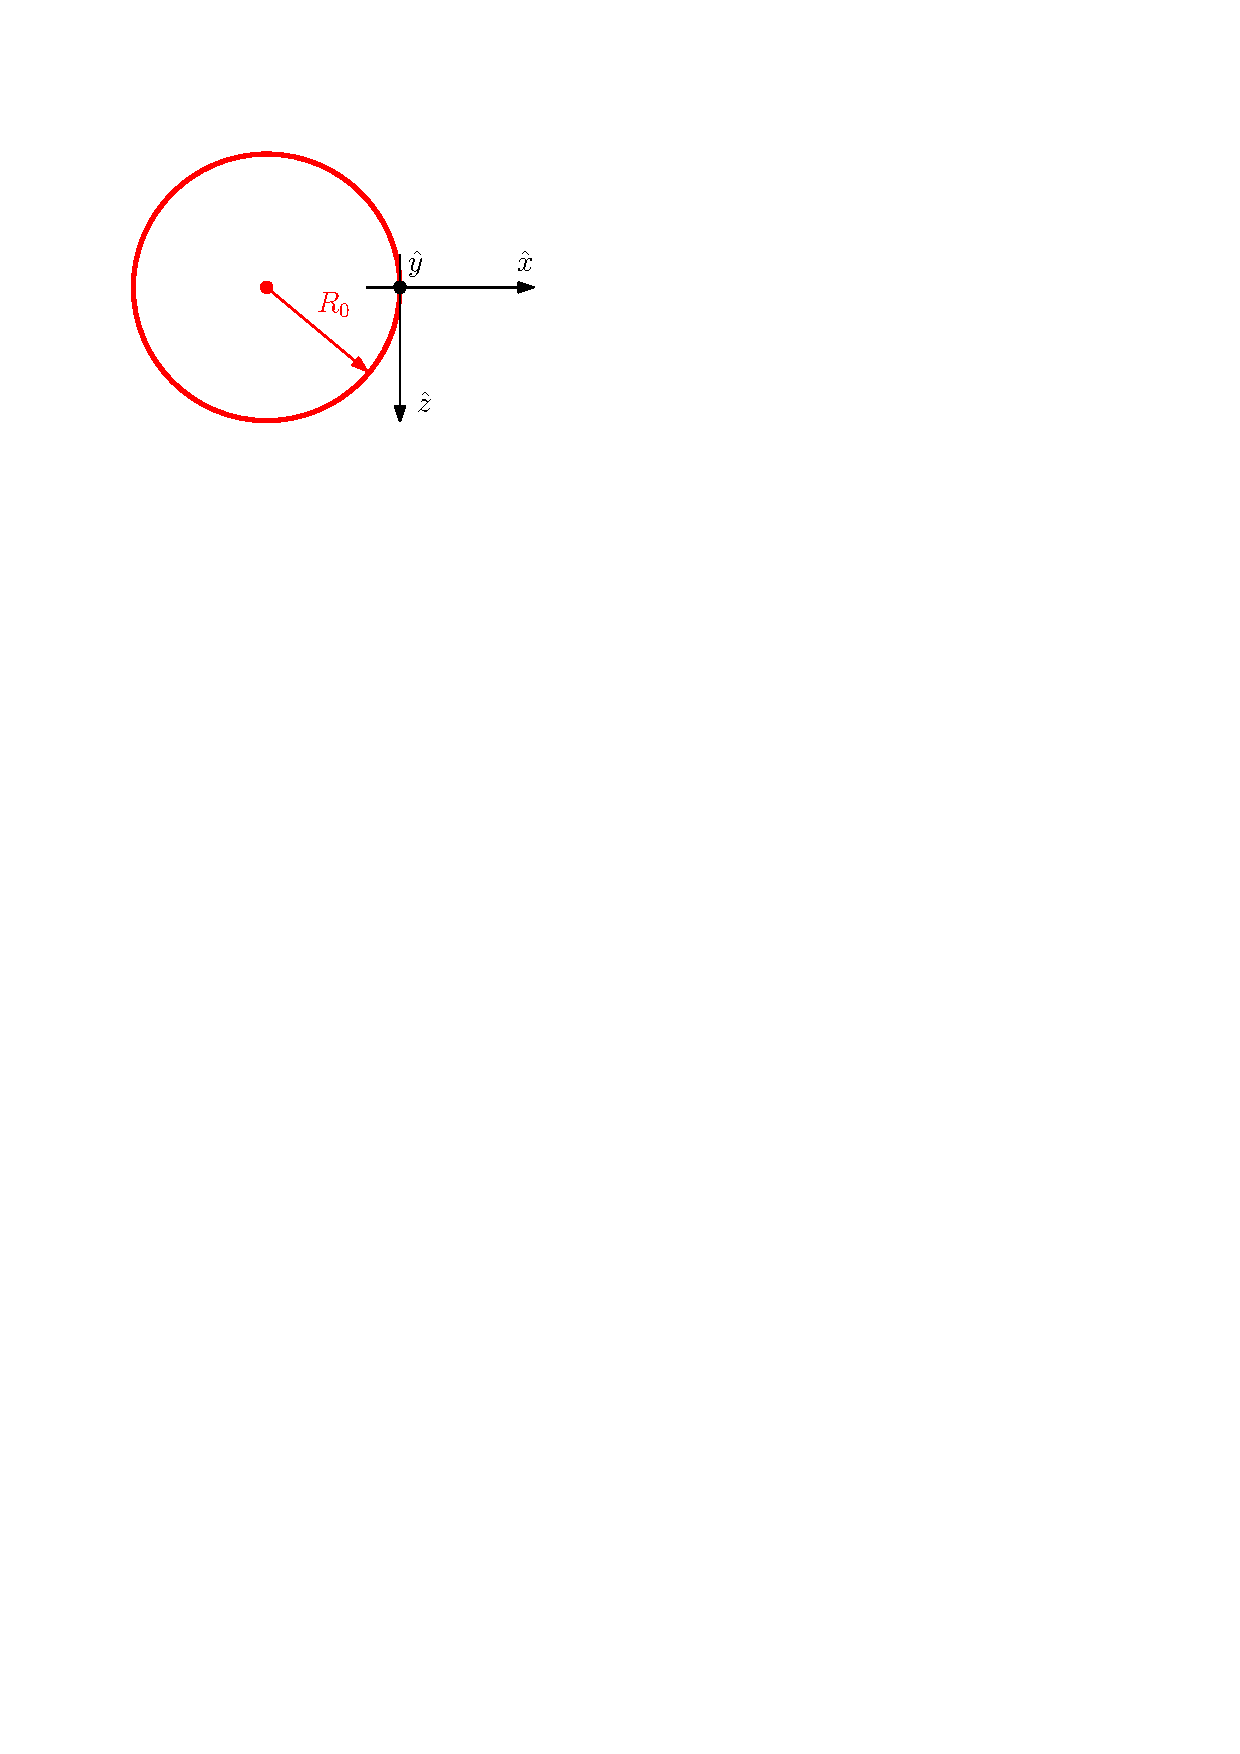
\includegraphics[width=0.5\textwidth]{figs/SPIgeom.pdf}
        \caption{
            Illustration of the coordinate system used for the SPI module in
            \DREAM.
        }
        \label{fig:geom}
    \end{figure}

    \section{Coordinate transformations}
    In the SPI module, it is necessary to map the cartesian coordinates
    $(x,y,z)$ of the points in space to the corresponding flux surface label
    $r$. In the toroidal case, this requires a two-step procedure where the
    cartesian coordinates $(x,y,z)$ are first transformed to their corresponding
    cylindrical $(R,Z,\varphi)$ or toroidal coordinates $(\rho,\theta,\varphi)$.
    In the second step, the cylindrical or toroidal coordinates must then be
    inverted to obtain the flux surface label $r$, and this generally requires
    numerical root-finding.

    \subsection{Cylindrical coordinates}
    The transformation to cylindrical coordinates is straightforward: since
    $x$ and $z$ lie in the horizontal plane, while $y$ is always vertical, the
    major radius and vertical position $Z$ is given by
    \begin{subequations}
        \begin{align}
        R &= \sqrt{x^2 + z^2},\\
        Z &= y.
        \end{align}
    \end{subequations}

    \subsection{Toroidal coordinates}
    To obtain the toroidal coordinates $\rho$ and $\theta$, we first introduce
    the position vector $\vec{r} = (x-R_0,y,z)$, defined to originate in $y=0$
    on the axis of symmetry of the tokamak (the red dot in
    figure~\ref{fig:geom}). We then introduce the unit vector
    \begin{equation}
        \hat{r} = \frac{\left(\vec{r}\cdot\hat{x}\right)\hat{x} + \left(\vec{r}\cdot\hat{z}\right)\hat{z}}
        {\sqrt{\left(\vec{r}\cdot\hat{x}\right)^2 + \left(\vec{r}\cdot\hat{z}\right)^2}} =
        %
        \frac{(x-R_0)\hat{x} + z\hat{z}}{\sqrt{x^2+z^2}},
    \end{equation}
    which is the normalized projection of the position vector $\vec{r}$ to the
    horizontal plane. With these vectors, we can then obtain the minor radius
    vector $\vec{\rho}$ as
    \begin{equation}
        \vec{\rho} = \vec{r}-R_0\hat{r} =
        \left(x-R_0-\frac{(x-R_0)R_0}{\sqrt{\left(x-R_0\right)^2 + z^2}}\right)\hat{x}
        + y\hat{y}
        + \left(z-\frac{zR_0}{\sqrt{\left(x-R_0\right)^2 + z^2}}\right)\hat{z},
    \end{equation}
    and the magnitude of this vector is
    \begin{equation}
        \rho = \sqrt{
            \left(x-R_0-\frac{(x-R_0)R_0}{\sqrt{\left(x-R_0\right)^2 + z^2}}\right)^2
            + y^2
            + \left(z-\frac{zR_0}{\sqrt{\left(x-R_0\right)^2 + z^2}}\right)^2
        }.
    \end{equation}
    Knowing the minor radius $\rho$ corresponding to $(x,y,z)$ will get us only
    part of the way to determining the flux surface radius $r$. To fully
    determine it, we also need to know the poloidal angle $\theta$ of the
    cartesian coordinates. In numerical geometry, this is easy to obtain from
    the minor radius vector $\vec{\rho}$. By the definition of the poloidal
    angle $\theta$ in numerical toroidal geometry, we have
    \begin{equation}
        \tan\theta = \frac{\left(\vec{\rho}\cdot\hat{y}\right)\mathrm{sgn}\left(R-R_0\right)}
            {\sqrt{\left(\vec{\rho}\cdot\hat{x}\right)^2 + \left(\vec{\rho}\cdot\hat{z}\right)^2}}
        %
        = \frac{y\,\mathrm{sgn}\left(R-R_0\right)}{\sqrt{
            \left(x-R_0-\frac{(x-R_0)R_0}{\sqrt{\left(x-R_0\right)^2 + z^2}}\right)^2
            + \left(z-\frac{zR_0}{\sqrt{\left(x-R_0\right)^2 + z^2}}\right)^2
        }},
    \end{equation}
    with
    \begin{equation}
        R = \sqrt{(x-R_0)^2+z^2}.
    \end{equation}
    The sign function appears since
    $\sqrt{(\vec{\rho}\cdot\hat{x})^2 + (\vec{\rho}\cdot\hat{z})^2}$
    should correspond to the horizontal cartesian coordinate in the poloidal
    plane (which is negative in the second and third quadrants).
\end{document}
